\section{Outros}

\subsection{MUF - Make Union Find}
Também conhecido como DSU - Disjoint Set Union

Algoritmo relacionado a conectividade em grafos e algoritmos de agrupamento. Ex: uva793.cpp
\par Utilizado no algoritmo de Kruskal para Árvores Geradoras Mínimas.
\begin{verbatim}
    vi _p(MAX);
    vi _rank(MAX);

    int _find(int u){
        if (_p[u] == u) return u;
        return _p[u] = _find(_p[u]);
    }

    void _union(int u, int v){
        u = _find(u);
        v = _find(v);
        if (_rank[u] < _rank[v]) _p[u] = v;
        else{
            _p[v] = u;
            if (_rank[u] == _rank[v]) _rank[u]++;
        }
    }
\end{verbatim}

\par Antes de realizar as operações, utilizar as seguintes definições:
\begin{verbatim}
    for (int i = 0; i < n; i++) {_p[i]=i; _rank[i]=0;}
\end{verbatim}

\subsection{Arredondamentos}
    Podemos também, ajustar a quantidade de casas decimais da nossa saída. Com o comando
    setprecision determinamos para todas as saídas a quantidade de casas decimais, sendo 
    esse comando capaz de fazer o arredondamento correto.
    \begin{verbatim}
        cout<<fixed<<setprecision(qtd_casas_decimais);
        cout<<numero<<endl;
    \end{verbatim}  

\subsection{Math.h}
    A biblioteca Math.h fornece muitas ferramentas para o trabalho com números, segue abaixo 
    uma tabela com seus principais comandos.

    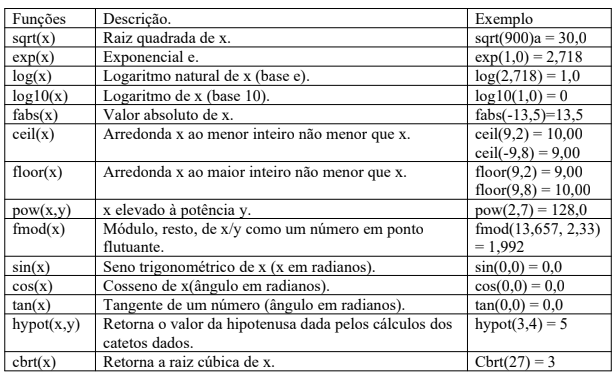
\includegraphics[width=130mm]{12_outros/ComandosMath.png}
    \pagebreak
    